%%%%%%%%%%%%%%%%%%%%%%%%%%%%%%%%%%%%%%%%%%%%%%%%%%%%%%%%%%%%%%%%%%%%%%
% How to use writeLaTeX: 
%
% You edit the source code here on the left, and the preview on the
% right shows you the result within a few seconds.
%
% Bookmark this page and share the URL with your co-authors. They can
% edit at the same time!
%
% You can upload figures, bibliographies, custom classes and
% styles using the files menu.
%
%%%%%%%%%%%%%%%%%%%%%%%%%%%%%%%%%%%%%%%%%%%%%%%%%%%%%%%%%%%%%%%%%%%%%%

\documentclass[12pt]{article}

\usepackage{sbc-template}

\usepackage{graphicx,url}

\usepackage[brazilian]{babel}   
\usepackage[T1]{fontenc} % Codificação para fontes com suporte a caracteres acentuados
\usepackage[utf8]{inputenc} % Codificação UTF-8 (necessário apenas para pdflatex)
\usepackage{multicol}
\usepackage{amsmath,amssymb,amsfonts}
\usepackage{algorithmic}
\usepackage{textcomp}
\usepackage{enumerate}
\usepackage{multirow}
\usepackage{verbatim}
\usepackage[table,xcdraw]{xcolor}
\usepackage[shortlabels]{enumitem}
\usepackage{scalefnt} % pacote para diminuir fonte das tabelas
\usepackage{comment} % pacote de comentarios
\usepackage{lscape}
\usepackage{fancyhdr}
\usepackage{IHC}
\usepackage[super]{nth}
\usepackage{pdfcomment}
\usepackage{float}
\usepackage{xurl}
\usepackage{booktabs}
\usepackage{array}
\usepackage{tikz}
\usetikzlibrary{shapes.geometric, arrows.meta, positioning, fit}


%By IHC 2026: package to insert description in images | pacote para inserir descrição nas imagens

%previne hifenização
\tolerance=1
\emergencystretch=\maxdimen
\hyphenpenalty=10000
\hbadness=10000

\sloppy


\trilha{Pesquisa} %Preencha com: Pesquisa | Ideias Inovadoras e Resultados Emergentes | Relatos de Experiência | Prêmio Junia Coutinho Anacleto | Pôsteres, Demonstrações e Artigos Internacionais | WTD ! Minicursos e Workshops | Competição de Avaliação | IHC na Prática | WEIHC | WAIHCWS
\local{Quixadá/CE} 
\ano{2026} 
\edicao{XXV} 

\title{Interação Humano-Dados em Contextos Urbanos: Uma Revisão Sistemática da Literatura} %deve ser no mesmo idioma do texto

\author{Autor anônimo 1, Autor anônimo 2}

\address{Endereço anônimo\\
  Estado anônimo -- País anônimo
  \email{Endereço eletrônico anônimo 1, Endereço eletrônico anônimo 2}}


\begin{document} 

%%  ATENÇÃO: AS INFORMAÇÕES DESTACADAS EM AZUL SÃO APENAS PARA INFORMAR OS AJUSTES NO TEMPLATE DA SBC E ACRESCENTAR INSTRUÇÕES DE ACESSIBILIDADE. O SEU TEXTO NÃO DEVE ESTAR NA COR AZUL.

\maketitle

\thispagestyle{plain}

%CAMPO OBRIGATÓRIO NESTE FORMATO.
\begin{abstract}{
\textbf{Introduction:} Smart cities' growing datafication demands systems that respect citizen privacy and autonomy; Human-Data Interaction (HDI) responds through legibility, agency, and negotiability. \textbf{Objective:} Map HDI's evolution in urban contexts (2014--2024). \textbf{Methodology:} A Systematic Literature Review following PRISMA yielded a \textit{corpus} of 98 studies. \textbf{Results:} Findings show a shift from technical to sociotechnical concerns, yet gaps persist (missing design guidelines and cognitive overload); mapped frameworks are organized into a comparative matrix and a taxonomy by HDI pillar. HDI proves fundamental to democratic urban governance, aligning with GC5 of GranDIHC-BR.}
\end{abstract}

\keywords{Human-Data Interaction (HDI), Smart Cities, Data Governance, Data Privacy, Data Literacy.}
     

%ATENÇÃO PESSOAS AUTORAS
\begin{resumo}{
  \textbf{Introdução:} A dataficação em cidades inteligentes exige sistemas que respeitem a privacidade e a autonomia do cidadão; a IHD responde promovendo legibilidade, agência e negociabilidade. \textbf{Objetivo:} Mapear a evolução da IHD em contextos urbanos (2014--2024). \textbf{Metodologia:} Uma Revisão Sistemática da Literatura seguindo o protocolo PRISMA resultou em \textit{corpus} de 98 trabalhos. \textbf{Resultados:} Os achados evidenciam transição de preocupações técnicas para sociotécnicas, mas persistem lacunas (diretrizes de projeto e sobrecarga cognitiva); os \textit{frameworks} mapeados são organizados em uma matriz comparativa e em uma taxonomia por pilar da IHD. A IHD mostra-se fundamental para governança urbana mais democrática, alinhando-se ao GC5 do GranDIHC-BR.}
\end{resumo}

\palavraschave{Interação Humano-Dados (IHD), Cidades Inteligentes, Governança de Dados, Privacidade de Dados, Letramento de Dados.}


\section{Introdução}

    A urbanização tem avançado rapidamente ao longo do século XXI, com projeções da ONU indicando que mais de 60\% da população global viverá em cidades,\footnote{Disponível em: https://brasil.un.org/pt-br/188520-onu-habitat-população-mundial-será-68-urbana-até-2050. Acesso em: 20 maio 2026.} impulsionando a busca por soluções inteligentes e sustentáveis. Em resposta a essa demanda, a comunidade científica, a indústria e a esfera política passaram a tratar as Cidades Inteligentes (\textit{Smart Cities}) como prioridade \cite{EREMIA2017}. Esses ecossistemas utilizam tecnologias como Internet das Coisas (IoT) e Urbanismo de Plataforma, frequentemente com \textit{smartphones} atuando como sensores passivos, para otimizar serviços urbanos essenciais. Essa mesma infraestrutura, no entanto, enfrenta desafios críticos de privacidade e segurança devido à coleta massiva de dados (dataficação), muitas vezes realizada sob a premissa de um consentimento presumido, sem transparência ou controle efetivo pelos cidadãos \cite{streitz2019beyond}.

   Diante dessa assimetria estrutural, o paradigma da Interação Humano-Dados (IHD) surge como uma abordagem ética e centrada no usuário para reequilibrar a relação entre indivíduos e sistemas invisíveis, apoiando-se nos pilares de legibilidade, agência e negociabilidade propostos por \cite{mortier2015humandatainteractionhumanface}, detalhados na Seção~\ref{sec:referencial}.

    Apesar de o arcabouço da IHD se apresentar na literatura como uma perspectiva promissora para o reequilíbrio dessas dinâmicas, sua aplicação empírica enfrenta limitações práticas e socioculturais expressivas \cite{Victorelli2020Human}, persistentes mesmo em estudos recentes conduzidos em contextos conectados \cite{DOWTHWAITE2024} e comunitários \cite{hayes2024making}. As pesquisas incorporadas a esta revisão apontam lacunas, como a dificuldade de engajamento dos usuários leigos no \textit{design} de sistemas e a ausência de clareza em contratos de uso de dados \cite{Victorelli2020Human}. Este problema é especialmente grave para populações vulneráveis e marginalizadas, que enfrentam risco desproporcional de discriminação e exclusão diante de tecnologias orientadas a dados, muitas vezes sem letramento ou recursos suficientes para compreender plenamente as ramificações de vigilância a que estão sujeitas \cite{malgieri2020vulnerable, hayes2024making}. Além disso, fatores contextuais intrínsecos a cada região, como disparidades culturais, letramento de dados e ambiguidades interpretativas, influenciam diretamente como os dados são gerenciados e compartilhados \cite{Yuan20243615, Belizario2023Interacao}, exigindo abordagens mais inclusivas e geopoliticamente situadas para que a interação humano-dados seja ética e transparente \cite{Elhamdadi2022}.

    Diante desse cenário, este artigo apresenta uma Revisão Sistemática da Literatura (RSL) com o objetivo de mapear como os princípios de Interação Humano-Dados (legibilidade, agência e negociabilidade) \cite{mortier2015humandatainteractionhumanface} têm sido abordados em pesquisas sobre aplicações urbanas na última década. Este trabalho mapeia o estado da arte, as tendências teóricas e as lacunas que ainda impedem uma gestão de dados mais transparente e centrada no cidadão. Os resultados desta revisão oferecem subsídios para pesquisadores e \textit{designers} de sistemas urbanos, dialogando com os Grandes Desafios de Pesquisa em Interação Humano-Computador no Brasil (GranDIHC-BR-2025-2035), em especial ao GC5 (Interação Humano-Dados, Alfabetização em Dados e Privacidade Utilizável), foco desta revisão ao investigar lacunas de privacidade e letramento de dados em ecossistemas emergentes.

    As principais contribuições deste artigo são: (i) uma síntese da evolução histórica e conceitual da IHD entre 2014 e 2024, articulando os pilares de legibilidade, agência e negociabilidade; (ii) o mapeamento de lacunas estruturais, cognitivas e socioculturais que ainda dificultam a aplicação prática da IHD em contextos urbanos; (iii) uma matriz comparativa de \textit{frameworks}, contextos de validação empírica e métodos de avaliação; e (iv) uma taxonomia que organiza esses \textit{frameworks} pelos três pilares da IHD, subsídio para trabalhos futuros na área.

    Para o alcance dessas metas, este trabalho adota uma abordagem metodológica de natureza teórica e descritiva. O procedimento analítico foi estruturado a partir de um protocolo de mapeamento organizado em três fases fundamentais: o planejamento (delineamento das questões de pesquisa e calibração das \textit{strings} de busca), a execução (varredura nas bases de dados e aplicação dos critérios de elegibilidade) e a análise crítica (extração, categorização e síntese qualitativa das evidências), conforme detalhado na seção a seguir.
    

\section{Fundamentação teórica}
\label{sec:referencial}

Esta seção apresenta, de forma sucinta, as bases conceituais que fundamentam esta revisão, retomadas na análise crítica da Seção~\ref{sec:resultados}.

\subsection{Interação Humano-Dados}

A Interação Humano-Dados (IHD) foi proposta em 2015 como um campo autônomo, distinto da Interação Humano-Computador (IHC) clássica, por deslocar o foco da usabilidade de interfaces visíveis para a relação ética entre o indivíduo e seus rastros de dados processados de forma frequentemente invisível \cite{mortier2015humandatainteractionhumanface}. Esse marco fundacional é adotado nesta revisão como o divisor temporal entre o período ``pré-IHD'' \cite{Mashhadi2014} e a emergência da área como campo interdisciplinar próprio \cite{Sailaja2021Designing}.

O modelo de \cite{mortier2015humandatainteractionhumanface} estrutura-se em três pilares: a \textbf{legibilidade}, entendida como a capacidade do usuário de compreender e construir sentido (\textit{sensemaking}) sobre os dados coletados e os algoritmos que os processam; a \textbf{agência}, que corresponde ao papel ativo do cidadão como administrador de seus próprios rastros digitais, com poder real de decisão sobre sua participação em ecossistemas datificados; e a \textbf{negociabilidade}, que trata da possibilidade de revisão e revogação dinâmica de permissões conforme o contexto social e urbano se transforma.

\section{Metodologia} \label{sec:metodologia}

    Esta seção detalha o protocolo metodológico da Revisão Sistemática da Literatura (RSL), conduzida segundo diretrizes consolidadas para revisões sistemáticas em Computação \cite{KITCHENHAM2013} e o protocolo PRISMA 2020 \cite{prisma2021}, ilustrado na Figura~\ref{fig:prisma_flow}. O objetivo é mapear o estado da arte da Interação Humano-Dados (IHD) em contextos urbanos, focando na evolução dos princípios de legibilidade, agência e negociabilidade na última década. O processo busca conferir rigor e reprodutibilidade desde a formulação das questões de pesquisa até a síntese das evidências, visando consolidar práticas recorrentes e identificar lacunas teóricas que fundamentem pesquisas futuras em cenários de cidades inteligentes.

    \begin{figure}[H]
    \centering
    \resizebox{\linewidth}{!}{%
    \begin{tikzpicture}[
      font=\scriptsize,
      stage/.style={rectangle, fill=blue!70!black, text=white, font=\bfseries\scriptsize, text width=1.6cm, align=center, minimum height=2.4cm},
      main/.style={rectangle, draw=blue!50!black, fill=blue!8, rounded corners, text width=7cm, align=left, inner sep=6pt},
      mainGreen/.style={rectangle, draw=green!40!black, fill=green!12, rounded corners, text width=7cm, align=left, inner sep=6pt},
      side/.style={rectangle, draw, rounded corners, text width=6.6cm, align=left, inner sep=6pt},
      arrow/.style={-{Latex[length=2.5mm]}, thick}
    ]

    \node[font=\bfseries\normalsize] (title) {Fluxo de Seleção dos Estudos---PRISMA 2020};

    % Linha 1: Identificação
    \node[main, below=0.6cm of title] (id) {\textbf{Registros identificados nas bases de dados (n = 268)}\\
    Scopus (n = 193) \quad Science Direct (n = 52)\\
    Portal de Periódicos CAPES (n = 14)\\
    Catálogo de Teses CAPES (n = 7) \quad BDTD-USP (n = 2)};

    \node[stage, left=0.4cm of id] (s1) {IDENTIFI-\\CAÇÃO};

    \node[side, draw=orange!70!black, fill=orange!8, right=2.6cm of id] (filtros) {
    \textbf{Parâmetros da busca na origem}\\
    $\bullet$ \textit{TITLE-ABS-KEY} = ``Human-Data Interaction''\\
    $\bullet$ Recorte temporal 2014--2024 (CI8), pré-aplicado na busca\\
    $\bullet$ Sem filtro de idioma (\textit{corpus} naturalmente em inglês/português)};

    % Linha 2: Triagem
    \node[main, below=1.8cm of id] (triagem) {\textbf{Registros submetidos à triagem (n = 268)}\\
    Avaliação completa frente aos critérios\\
    de inclusão (CI1--CI8) e exclusão (CE1--CE9).};

    \node[stage, left=0.4cm of triagem] (s2) {TRIAGEM};

    \node[side, draw=red!60!black, fill=red!8, right=2.6cm of triagem] (excluidos) {
    \textbf{Registros excluídos na triagem (n = 170)}\\
    Motivos predominantes (categorias não exclusivas):\\
    $\bullet$ CE2---menção superficial à IHD\\
    $\bullet$ CE8---uso estritamente clínico\\
    $\bullet$ CE4---hardware / interação de baixo nível\\
    Portal de Periódicos CAPES e BDTD-USP: exclusão total por duplicatas (CE9) já retidas no Scopus.};

    % Linha 3: Elegibilidade
    \node[main, below=2.1cm of triagem] (eleg) {\textbf{Estudos avaliados quanto à elegibilidade (n = 98)}\\
    Leitura na íntegra e Avaliação de Qualidade (AQ)\\
    em escala de 0 a 3 pontos.};

    \node[stage, left=0.4cm of eleg] (s3) {ELEGIBILI-\\DADE};

    \node[side, draw=green!50!black, fill=green!8, right=2.6cm of eleg] (aq) {
    \textbf{Resultado da Avaliação de Qualidade}\\
    $\bullet$ AQ = 0 $\rightarrow$ 0 estudos (0,0\%)\\
    $\bullet$ AQ = 1 $\rightarrow$ 30 estudos (30,6\%)\\
    $\bullet$ AQ = 2 $\rightarrow$ 27 estudos (27,6\%)\\
    $\bullet$ AQ = 3 $\rightarrow$ 41 estudos (41,8\%)\\
    AQ usada como indicador de cobertura temática, não como filtro---todos os 98 seguiram para extração e análise integral.};

    % Linha 4: Inclusão
    \node[mainGreen, below=2.1cm of eleg] (inc) {\textbf{Estudos incluídos no \textit{corpus} final (n = 98)}\\
    Scopus (n = 81) \quad Science Direct (n = 14)\\
    Catálogo de Teses CAPES (n = 3)\\
    Periódicos CAPES (n = 0) \quad BDTD-USP (n = 0)\\
    Cobertura temporal: 2014--2024 (pico 2020--2021).};

    \node[stage, left=0.4cm of inc] (s4) {INCLUSÃO};

    % Fluxo principal
    \draw[arrow] (id.south) -- (triagem.north);
    \draw[arrow] (triagem.south) -- (eleg.north);
    \draw[arrow] (eleg.south) -- (inc.north);

    % Fluxo para caixas laterais
    \draw[arrow, color=orange!70!black] (id.east) -- (filtros.west);
    \draw[arrow, color=red!60!black] (triagem.east) -- (excluidos.west);
    \draw[arrow, color=green!50!black] (eleg.east) -- (aq.west);

    \end{tikzpicture}}
    \caption{Fluxo de seleção dos estudos seguindo o protocolo PRISMA 2020. O diagrama apresenta quatro etapas verticais conectadas por setas. Na etapa de Identificação, 268 registros foram identificados em cinco bases (Scopus 193, Science Direct 52, Portal de Periódicos CAPES 14, Catálogo de Teses CAPES 7, BDTD-USP 2), com filtro automático de \textit{string} de busca e recorte temporal 2014--2024 aplicados na origem, sem filtro de idioma (\textit{corpus} naturalmente em inglês/português). Na etapa de Triagem, os 268 registros foram avaliados pelos critérios de inclusão CI1--CI8 e exclusão CE1--CE9, resultando em 170 exclusões, predominantemente por menção superficial à IHD, uso clínico ou \textit{hardware} de baixo nível; o Portal de Periódicos CAPES e a BDTD-USP tiveram exclusão total por duplicatas já retidas no Scopus. Na etapa de Elegibilidade, os 98 estudos remanescentes foram lidos na íntegra e avaliados quanto à qualidade (30 estudos com pontuação 1, 27 com pontuação 2, 41 com pontuação 3, nenhum com pontuação 0), usada como indicador de cobertura temática e não como filtro de exclusão. Na etapa de Inclusão, o \textit{corpus} final de 98 estudos distribui-se em Scopus (81), Science Direct (14) e Catálogo de Teses CAPES (3), com cobertura temporal de 2014 a 2024 e pico de publicações em 2020--2021.}
    \label{fig:prisma_flow}
\end{figure}

\subsection{Fontes de dados}

    Para a revisão sistemática, esta pesquisa utilizou fontes diversificadas que incluem bases internacionais e nacionais de relevância acadêmica. A \emph{Scopus\footnote{Disponível em: https://www.scopus.com. Acesso em: 20 maio 2026.}} foi selecionada como fonte principal devido ao seu escopo multidisciplinar, essencial para mapear a interseção entre tecnologia e o contexto urbano, e por indexar de forma agregada o conteúdo de editoras como Elsevier, ACM e IEEE. Ainda assim, reconhece-se que essa escolha pode ter deixado de fora trabalhos indexados apenas em bases nativas como a ACM Digital Library e a IEEE Xplore. A cobertura da Scopus sobre a Biblioteca Digital da SBC (SOL) é seletiva e curada por evento/periódico via seu \textit{Content Selection Advisory Board} (CSAB), de modo que trabalhos publicados em veículos da SOL ainda não admitidos nesse processo de curadoria podem não estar indexados. Para mitigar essa lacuna pontual, a busca foi complementada com consultas diretas ao Portal de Periódicos CAPES, ao Catálogo de Teses CAPES e à BDTD-USP, capturando produção acadêmica brasileira independentemente de sua indexação na Scopus, limitação retomada na Seção~\ref{sec:ameacas}.

    Adicionalmente, foram consultadas bases especializadas como o \emph{Science Direct\footnote{Disponível em: https://www.sciencedirect.com. Acesso em: 20 maio 2026.}} para acesso a publicações técnicas, dado seu peso editorial na literatura de urbanismo e sistemas ciberfísicos, e o \emph{Portal de Periódicos CAPES\footnote{Disponível em: https://www.periodicos.capes.gov.br. Acesso em: 20 maio 2026.}} para a inclusão de produção científica nacional. Para abranger pesquisas acadêmicas brasileiras relevantes, incluindo teses e dissertações não necessariamente publicadas em periódicos indexados pela Scopus, foram utilizados os \emph{Repositórios de Teses da USP\footnote{Disponível em: https://www.teses.usp.br. Acesso em: 20 maio 2026.}} e da \emph{CAPES\footnote{Disponível em: https://catalogodeteses.capes.gov.br. Acesso em: 20 maio 2026.}}.
    
    %Para a revisão sistemática, esta pesquisa utilizou fontes diversificadas que incluem bases internacionais e nacionais de relevância acadêmica reconhecida. A \emph{Scopus\footnote{Disponível em: https://www.scopus.com. Acesso em: 20 maio 2026.}} foi selecionada como fonte principal por seu amplo escopo, indexando artigos de alto impacto de editoras como Elsevier, IEEE Xplore e ACM Digital Library, além de oferecer cobertura de periódicos internacionais.

   %Adicionalmente, foram consultadas bases especializadas como o \emph{Science Direct\footnote{Disponível em: https://www.sciencedirect.com. Acesso em: 20 maio 2026.}} para acesso a publicações técnicas, e o \emph{Portal de Periódicos CAPES\footnote{Disponível em: https://www.periodicos.capes.gov.br. Acesso em: 20 maio 2026.}} para a inclusão de produção científica nacional. Para abranger pesquisas acadêmicas brasileiras relevantes, foram utilizados os \emph{Repositórios de Teses da USP\footnote{Disponível em: https://www.teses.usp.br. Acesso em: 20 maio 2026.}} e da \emph{CAPES\footnote{Disponível em: https://catalogodeteses.capes.gov.br. Acesso em: 20 maio 2026.}}.

\subsection{Período de Publicação}

   O período selecionado compreende os anos de 2014 a 2024, intervalo que acompanha a emergência da IHD como campo de estudo distinto. O marco inicial remete ao surgimento do termo na literatura acadêmica, impulsionado por trabalhos fundacionais \cite{mortier2015humandatainteractionhumanface,Hornung2015}, que estabeleceram as bases da relação entre humanos e dados pessoais. Esta década permite rastrear desde a fundamentação teórica inicial até os estudos recentes que dialogam com as regulamentações globais de proteção de dados, como o Regulamento Geral de Proteção de Dados (GDPR) \cite{gdpr2016}, refletindo os desafios contemporâneos da IHD no urbanismo de plataforma \cite{Belizario2023Interacao,chalhoub2024useful,coleti2024grandihc}.

\subsection{Questões de Pesquisa}

 Esta revisão sistemática foi estruturada a partir de um conjunto de questões, elaboradas para mapear o estado da arte da Interação Humano-Dados (IHD) e identificar os desafios emergentes na área. As questões foram divididas em principais e secundárias:

\textbf{Questões Principais (QP):}
\begin{itemize}
\item \textbf{QP1} - Como a literatura sobre Interação Humano-Dados (IHD) evoluiu em conceito e prática na última década (2014-2024)?
\item \textbf{QP2} - Quais são as principais diferenças entre as abordagens teóricas e as implementações práticas relatadas na literatura nesse período?
\item \textbf{QP3} - Quais lacunas na pesquisa atual são recorrentemente citadas nos estudos?
\item \textbf{QP4} - Antes da emergência da IHD, tomando como marco divisor o trabalho fundacional de \cite{mortier2015humandatainteractionhumanface} em 2015, conforme detalhado na Seção~\ref{sec:referencial}, quais abordagens facilitavam o entendimento sobre a gestão de dados em aplicações?
\item \textbf{QP5} - Qual é a importância da aplicação da IHD no contexto de \textit{Smart Cities}?
\end{itemize}

\textbf{Questões Secundárias (QPS):}
\begin{itemize}
\item \textbf{QPS1} - Quais métodos de avaliação (ex.: testes de usabilidade, \textit{eye-tracking}) são usados para medir a eficácia da IHD?
\item \textbf{QPS2} - Quais elementos de sistemas IHD ajudam usuários inexperientes digitalmente a compreender melhor os dados?
\item \textbf{QPS3} - Os estudos de caso analisados testaram algum \textit{framework} utilizando IHD?
\item \textbf{QPS4} - De que forma fatores étnico-culturais podem influenciar a aplicação da IHD?
\end{itemize}

Para fundamentar a busca e a seleção dos estudos destinados a responder a essas questões, o escopo da revisão foi delimitado utilizando uma adaptação da estrutura PICOC---do inglês Population, Intervention, Control, Outcomes, and Context (População, Intervenção, Controle, Resultados e Contexto/Aplicação):

\begin{itemize}
\item \textbf{População:} Trabalhos acadêmicos da área de IHD e pesquisas que demonstrem aplicações concretas dos seus princípios em diversos contextos (termos de busca: \textit{``Human-Data Interaction''}, \textit{``HDI''}).
\item \textbf{Intervenção:} Delimitação do escopo conceitual da IHD, mapeamento dos princípios teóricos fundamentais, metodologias de mensuração aplicáveis e identificação de lacunas (termos: \textit{``framework''}, \textit{``legibility''}, \textit{``agency''}, \textit{``negotiability''}).
\item \textbf{Controle:} Seleção sistemática priorizando trabalhos que proponham (re)formulações de princípios de IHD, apresentem aplicações práticas ou discutam métodos de avaliação (termos: \textit{``case study''}, \textit{``evaluation method''}).
\item \textbf{Resultados:} Sistematização do conhecimento sobre métodos e técnicas empregados e o mapeamento das lacunas frequentes na literatura (termos: \textit{``usability''}, \textit{``quality assessment''}).
\item \textbf{Aplicação:} Pesquisadores de IHD e IHC, além de profissionais da indústria que buscam compreender a aplicação e mensuração desses princípios na prática (termos: \textit{``smart cities''}, \textit{``urban''}).
\end{itemize}

\subsection{Estratégia de Busca e Elegibilidade}
\label{estrategiaDeBusca}

    A estratégia de identificação dos estudos integrou parâmetros temáticos e cronológicos. Esta pesquisa estabeleceu uma \textit{string} de busca base focada no termo ``Human-Data Interaction''; no caso da Scopus, a busca incidiu sobre título, resumo e palavras-chave (de acordo com o parâmetro \textit{TITLE-ABS-KEY}). Com vistas à reprodutibilidade, frente aos limites de formatação do artigo, o detalhamento das bucas em todas as bases, incluindo parâmetros de indexação e recortes temporais, está documentado e disponibilizado integralmente em um \emph{repositório suplementar}\footnote{Disponível em: https://anonymous.4open.science/r/sbc-rs-4046/Listas/Lista\%20de\%20Strings.txt. Acesso em: 20 maio 2026.}. O limite temporal da última década (2014--2024) foi parametrizado diretamente nos filtros de todas as bases, abrangendo desde os marcos conceituais pioneiros da área (Seção~\ref{sec:referencial}) até os desenvolvimentos mais recentes.

    Foram elegíveis contribuições teóricas (\textit{frameworks} e princípios), artigos metodológicos sobre mensuração de usabilidade, estudos de caso em soluções urbanas e revisões sistemáticas correlatas. Não foi aplicado filtro de idioma em nenhuma etapa da busca ou triagem; o \textit{corpus} resultante concentrou-se naturalmente em inglês e português, consequência do termo de busca ``Human-Data Interaction'' ser de origem anglófona e da inclusão de bases brasileiras (Portal de Periódicos CAPES, Catálogo de Teses CAPES e BDTD-USP) na estratégia de busca.
    
%A estratégia de identificação dos estudos integrou parâmetros temáticos e cronológicos. Estabeleceu-se uma \textit{string} de busca base focada no termo ``Human-Data Interaction'', configurada inicialmente para a base Scopus—incidindo sobre título, resumo e palavras-chave (\textit{TITLE-ABS-KEY}). Esta equação principal foi adaptada à sintaxe específica e às regras de indexação de cada uma das outras plataformas, sendo as \textit{strings} exatas de cada repositório detalhadas no Apêndice A (ou Tabela X). O limite temporal da última década (2014-2024) foi parametrizado diretamente nos filtros de todas as bases, abrangendo desde os marcos conceituais pioneiros até os desenvolvimentos mais recentes da área.
%A estratégia de identificação dos estudos integrou parâmetros temáticos e cronológicos. Estabeleceu-se uma \textit{string} de busca base focada no termo ``Human-Data Interaction'', configurada inicialmente para a base Scopus—incidindo sobre título, resumo e palavras-chave (\textit{TITLE-ABS-KEY}). Esta equação principal foi adaptada à sintaxe específica e às regras de indexação de cada uma das outras plataformas. O limite temporal da última década (2014-2024) foi parametrizado diretamente nos filtros de todas as bases, abrangendo desde os marcos conceituais pioneiros até os desenvolvimentos mais recentes da área\footnote{Disponível em: https://anonymous.4open.science/r/sbc-rs-4046/Listas/Scopus\_Lista\%20de\%20artigos.txt. Acesso em: 20 maio 2026.}\footnote{Disponível em: https://anonymous.4open.science/r/sbc-rs-4046/Listas/Sicence\%20Direct\_Lista\%20de\%20artigos.txt. Acesso em: 20 maio 2026.}\footnote{Disponível em: https://anonymous.4open.science/r/sbc-rs-4046/Listas/Periódicos\%20Capes\_Lista\%20de\%20artigos.txt. Acesso em: 20 maio 2026.}\footnote{Disponível em: https://anonymous.4open.science/r/sbc-rs-4046/Listas/Teses\%20USP\_Lista\%20de\%20Teses.txt. Acesso em: 20 maio 2026.}\footnote{Disponível em: https://anonymous.4open.science/r/sbc-rs-4046/Listas/Teses\%20Capes\_Lista\%20de\%20teses.txt. Acesso em: 20 maio 2026.}.

%Foram elegíveis contribuições teóricas (\textit{frameworks} e princípios), artigos metodológicos sobre mensuração de usabilidade, estudos de caso em soluções urbanas e revisões sistemáticas correlatas. Quanto ao idioma, embora sem restrições formais iniciais, priorizaram-se publicações em inglês e português, escolha justificada pela predominância do inglês na literatura científica global e pela relevância do português para o contexto de aplicação urbano brasileiro que motiva esta pesquisa.

\subsection{Critérios de Seleção e Avaliação de Qualidade}

  Para estruturar a seleção dos estudos e sistematizar o conhecimento sobre o estado da arte em IHD no contexto urbano, foram estabelecidos critérios de inclusão (CI) e exclusão (CE), documentados nas \emph{tabelas resultantes da execução da RSL}\footnote{Disponível em: https://anonymous.4open.science/r/sbc-rs-4046/Tabelas/. Acesso em: 20 maio 2026.}. Esses parâmetros, detalhados na Tabela~\ref{tab:criterios}, buscam equilibrar  abrangência teórica e especificidade prática, priorizando trabalhos replicáveis, disponíveis na íntegra e alinhados ao recorte temporal (2014–2024).

\begin{table}[H]
\centering
\caption{Critérios de Inclusão (CI) e Exclusão (CE)}
\label{tab:criterios}
\scriptsize
\renewcommand{\arraystretch}{0.85}
\begin{tabular}{p{0.12\linewidth} p{0.8\linewidth}}
\hline
\textbf{Código} & \textbf{Descrição do Critério} \\
\hline
\multicolumn{2}{c}{\textbf{Critérios de Inclusão (CI)}} \\
\hline
\textbf{CI1} & Trabalhos que proponham, definam ou aprimorem princípios teóricos e fundamentais da IHD. \\
\textbf{CI2} & Estudos que apresentem a formulação ou aplicação prática de \textit{frameworks} baseados nesses princípios. \\
\textbf{CI3} & Pesquisas focadas no desenvolvimento, aplicação ou validação de métricas e métodos de avaliação em sistemas de IHD. \\
\textbf{CI4} & Artigos que relatem resultados empíricos (qualitativos ou quantitativos) acerca da eficácia e da usabilidade de soluções ou \textit{frameworks} de IHD. \\
\textbf{CI5} & Modelos teóricos sustentados e validados por evidências concretas, tais como estudos de caso e experimentos controlados. \\
\textbf{CI6} & Revisões sistemáticas e mapeamentos da literatura que ofereçam contribuições originais ou consolidações teóricas relevantes para a área. \\
\textbf{CI7} & Publicações submetidas a processo de revisão por pares (\textit{peer-review}), incluindo anais de conferências indexadas e periódicos acadêmicos. \\
\textbf{CI8} & Trabalhos publicados no período estabelecido para o levantamento metodológico, compreendendo os anos de 2014 a 2024. \\
\hline
\multicolumn{2}{c}{\textbf{Critérios de Exclusão (CE)}} \\
\hline
\textbf{CE1} & Trabalhos com metodologia não replicável ou que não apresentem uma descrição clara e rigorosa dos procedimentos adotados. \\
\textbf{CE2} & Artigos que citem a IHD de maneira apenas tangencial ou superficial, sem aprofundamento em seus princípios, \textit{frameworks} ou métricas. \\
\textbf{CE3} & Estudos focados exclusivamente em visualização de dados, mas que não abordem o componente ativo de interação humana. \\
\textbf{CE4} & Pesquisas que empreguem a sigla ou o termo atrelado à IHD em contextos não correlatos (como interfaces estritas de \textit{hardware} ou interações em baixo nível computacional). \\
\textbf{CE5} & Trabalhos publicados em período anterior a 2014, situando-se fora do recorte temporal delimitado para a revisão. \\
\textbf{CE6} & Documentos disponibilizados apenas em formato de resumo expandido, \textit{abstract}, ou cujos textos completos encontravam-se indisponíveis. \\
\textbf{CE7} & Documentos com texto integral indisponível gratuitamente (restritos a \textit{paywalls} ou bibliotecas pagas). \\
\textbf{CE8} & Artigos voltados estritamente à área médica ou clínica, afastando-se do escopo sociotécnico e urbano estabelecido por esta investigação. \\
\textbf{CE9} & Registros duplicados nas bases de dados, sendo contabilizada para análise apenas a versão mais completa, recente ou indexada na base prioritária. \\
\hline
\end{tabular}
\end{table}

Após a filtragem por CI e CE, os estudos elegíveis foram submetidos a uma Avaliação de Qualidade (AQ), documentada nas \emph{tabelas da RSL}\footnote{Disponível em: https://anonymous.4open.science/r/sbc-rs-4046/Tabelas/. Acesso em: 20 maio 2026.}. Esta etapa avaliou a contribuição de cada artigo para as questões de pesquisa, utilizando um sistema de pontuação baseado na abrangência com que cada estudo cobre os temas principais da revisão, definidos pelas questões de pesquisa (QP e QPS)---que contemplam os princípios de IHD (legibilidade, agência e negociabilidade), sua aplicação em contextos urbanos (\textit{Smart Cities}) e a gestão de dados do usuário---conforme a Tabela~\ref{tab:qualidade}. Todos os 98 artigos do \textit{corpus} foram submetidos à extração de dados e à análise integral, sendo a pontuação de AQ utilizada não como filtro de exclusão, mas como indicador da profundidade de cobertura temática de cada estudo.

\begin{table}[H]
\centering
\caption{Sistema de Pontuação para Avaliação de Qualidade (AQ)}
\label{tab:qualidade}
\small
\begin{tabular}{c p{0.75\linewidth}}
\hline
\textbf{Pontos} & \textbf{Nível de Contribuição do Artigo} \\ 
\hline
\textbf{0} & Sem contribuição metodológica ou teórica relevante para as Questões de Pesquisa. \\ 
\hline
\textbf{1} & Aborda apenas um dos temas da pesquisa de forma isolada. \\ 
\hline
\textbf{2} & Relaciona adequadamente dois dos temas da pesquisa. \\ 
\hline
\textbf{3} & Integra três ou mais temas da pesquisa. \\ 
\hline
\end{tabular}
\end{table}

\subsection{Condução das Buscas e Triagem dos Estudos}

As buscas foram executadas nas cinco bases de dados selecionadas, adaptando-se a \textit{string} principal (``Human-Data Interaction'') e o recorte temporal (2014 a 2024) às especificidades sintáticas de cada base (ex.: uso do comando \texttt{PUBYEAR} na Scopus; substituição do operador \textit{TITLE-ABS-KEY} pelos campos equivalentes de título, resumo e palavras-chave na ScienceDirect e no Portal de Periódicos CAPES). A triagem por título e resumo e a aplicação dos critérios de inclusão/exclusão foram conduzidas por ambos os autores deste trabalho, em decisão conjunta e não isolada. Para reduzir a subjetividade da triagem inicial, a decisão de inclusão foi orientada pela pontuação sistemática dos artigos segundo a matriz de Avaliação de Qualidade (Tabela~\ref{tab:qualidade}), cujos registros individuais por artigo estão disponíveis no repositório suplementar\footnote{Disponível em: https://anonymous.4open.science/r/sbc-rs-4046/Tabelas/. Acesso em: 20 maio 2026.}, permitindo a auditoria externa dos critérios aplicados a cada estudo. Ainda assim, a ausência de uma dupla triagem independente e cega constitui uma limitação reconhecida do processo de seleção, discutida na Seção~\ref{sec:ameacas}.

O levantamento bruto inicial retornou um total de \textbf{268 documentos}. A aplicação dos critérios de elegibilidade resultou em um \textit{corpus} final de \textbf{98 trabalhos} aprovados para a etapa de extração de dados e leitura na íntegra. A Tabela \ref{tab:funil_selecao} consolida o funil de seleção detalhado por repositório.

\begin{table}[H]
\centering
\caption{Consolidação do Funil de Seleção de Estudos por Base de Dados}
\label{tab:funil_selecao}
\small
\begin{tabular}{p{0.40\linewidth} c c c}
\hline
\textbf{Base de Dados} & \textbf{Retorno Inicial} & \textbf{Excluídos} & \textbf{Incluídos} \\ \hline
Scopus & 193 & 112 & 81 \\
Science Direct & 52 & 38 & 14 \\
Portal de Periódicos CAPES & 14 & 14 & 0 \\
Catálogo de Teses CAPES & 7 & 4 & 3 \\
BDTD-USP & 2 & 2 & 0 \\ \hline
\textbf{Total} & \textbf{268} & \textbf{170} & \textbf{98} \\ \hline
\end{tabular}
\end{table}
\vspace{-0.1 cm} 

A análise das 170 exclusões mostrou predominância de trabalhos fora do escopo conceitual da IHD. As remoções concentraram-se em abordagens superficiais da IHD (\textbf{CE2}) ou no uso do acrônimo em contextos puramente médicos (\textbf{CE8}) e de \textit{hardware} de baixo nível (\textbf{CE4}). No Portal de Periódicos CAPES e na BDTD-USP, o índice de exclusão total deveu-se estritamente à sobreposição de duplicatas (\textbf{CE9}) já retidas na busca primária (Scopus). Esse comportamento sugere que a estratégia de busca alcançou cobertura adequada ao escopo definido, resultando em um \textit{corpus} final de 98 artigos relevantes para as questões de pesquisa.

Na Avaliação de Qualidade (AQ), em escala de 0 a 3 para avaliar a cobertura dos temas de interesse da revisão---como os princípios de IHD, as cidades inteligentes, a governança de dados e as questões sociotécnicas---nenhum trabalho obteve pontuação nula, o que é coerente com o critério de seleção adotado, que priorizou estudos alinhados a esses temas.

A Tabela~\ref{tab:resumo_qualidade} sintetiza a distribuição das pontuações de qualidade do acervo. A maior parcela alcançou a pontuação máxima \emph{3} (\textbf{41} estudos, 41,8\%), integrando três ou mais eixos temáticos. Os demais distribuíram-se entre a pontuação \emph{2} (\textbf{27} artigos, 27,6\%), que relaciona dois eixos, e a pontuação \emph{1} (\textbf{30} artigos, 30,6\%), restrita a um único eixo. A concentração de estudos nos níveis 2 e 3 (69,4\% do acervo) indica que a maior parte das publicações retidas articula mais de um dos eixos temáticos de interesse.

\begin{table}[H]
\centering
\caption{Resultados da Avaliação de Qualidade (AQ)}
\label{tab:resumo_qualidade}
\small
\begin{tabular}{p{0.55\linewidth} c c}
\hline
\textbf{Pontuação (Nível de Contribuição)} & \textbf{Quantidade} & \textbf{Percentual} \\
\hline
(0) Sem contribuição teórica ou metodológica relevante & 0 & 0,0\% \\
(1) Aborda apenas um tema principal isoladamente & 30 & 30,6\% \\
(2) Relaciona dois temas principais & 27 & 27,6\% \\
(3) Integra três ou mais temas principais  & 41 & 41,8\% \\
\hline
\textbf{Total} & \textbf{98} & \textbf{100,0\%} \\
\hline
\end{tabular}
\end{table}

Em síntese, com o \textit{corpus} definido, a pesquisa avançou para a análise destas publicações, visando responder às Questões de Pesquisa (QPs) e mapear o estado da arte e as lacunas da governança de dados em sistemas sociotécnicos urbanos.

\subsection{Análise da Triagem e Perfil da Literatura}

% A triagem inicial avaliou \textbf{268} documentos, resultando na inclusão de \textbf{102} trabalhos. Essa taxa de retenção de 38\% reflete a aplicação de um filtro rigoroso para consolidar um \textit{corpus} robusto. Majoritariamente, os estudos selecionados atenderam a múltiplos critérios simultâneos, articulando \textit{frameworks} práticos (\textbf{CI2}), validação por revisão por pares (\textbf{CI7}), resultados empíricos (\textbf{CI4}) e o desenvolvimento de métricas de avaliação (\textbf{CI3}). Essa convergência demonstra que a literatura em IHD já transita da fundamentação conceitual para aplicações validadas, fornecendo subsídios vitais para esta análise.

% O alinhamento ao recorte temporal da última década (2014-2024) (\textbf{CI6}) reflete a emergência recente do tema. A atualidade do acervo garante que os debates sobre legibilidade e agência estejam alinhados aos desafios contemporâneos de privacidade e governança de dados.

% Em contrapartida, as \textbf{166} exclusões seguiram padrões claros: concentraram-se em abordagens superficiais da IHD (\textbf{CE4}) ou no uso do acrônimo em contextos estritamente médicos e desvinculados da interação humana (\textbf{CE6}). A remoção rigorosa de duplicatas (\textbf{CE1}) e de documentos com barreiras de acesso completou o funil. Essa limpeza metodológica contribui para um referencial teórico centrado no usuário e no desenvolvimento de aplicações urbanas.

A triagem inicial avaliou \textbf{268} documentos, resultando na inclusão de \textbf{98} trabalhos. Essa taxa de retenção de 36,6\% resultou da aplicação dos critérios de elegibilidade. Parte expressiva dos estudos selecionados atendeu a múltiplos critérios de inclusão, articulando \textit{frameworks} práticos (\textbf{CI2}), validação por revisão por pares (\textbf{CI7}), resultados empíricos (\textbf{CI4}) e o desenvolvimento de métricas de avaliação (\textbf{CI3}). Essa convergência sugere que a literatura em IHD tem transitado da fundamentação conceitual para aplicações validadas, fornecendo subsídios relevantes para esta análise.

O recorte temporal adotado, referente à última década (2014--2024) (\textbf{CI8}), acompanha a emergência recente do tema. A análise da distribuição temporal do \textit{corpus}, sintetizada na Figura~\ref{fig:distribuicao_ano_fonte}, evidencia três fases distintas na trajetória da IHD aplicada a contextos urbanos. Entre 2014 e 2019, observa-se produção incipiente, com 19 trabalhos publicados ao longo de seis anos (19,4\% do \textit{corpus}). O biênio 2020-2021 concentra 33 artigos (33,7\%), pico que coincide temporalmente com a aceleração das pesquisas em dataficação urbana no contexto pandêmico e com a sedimentação de marcos regulatórios como o Regulamento Geral de Proteção de Dados (GDPR), em vigor desde 2018. Em 2022-2024, o volume de publicações varia entre 10 e 20 artigos por ano (46 trabalhos, 46,9\%), padrão sugestivo de crescimento contínuo da produção do campo, com pico em 2024. A predominância da Scopus em todos os anos (cerca de 82,7\% do \textit{corpus}) corrobora a opção metodológica descrita na Seção~\ref{estrategiaDeBusca}, enquanto a contribuição pontual das Teses CAPES (2019, 2023 e 2024) sinaliza a entrada gradual da produção brasileira no debate.

\begin{figure}[H]
    \centering
    \pdftooltip{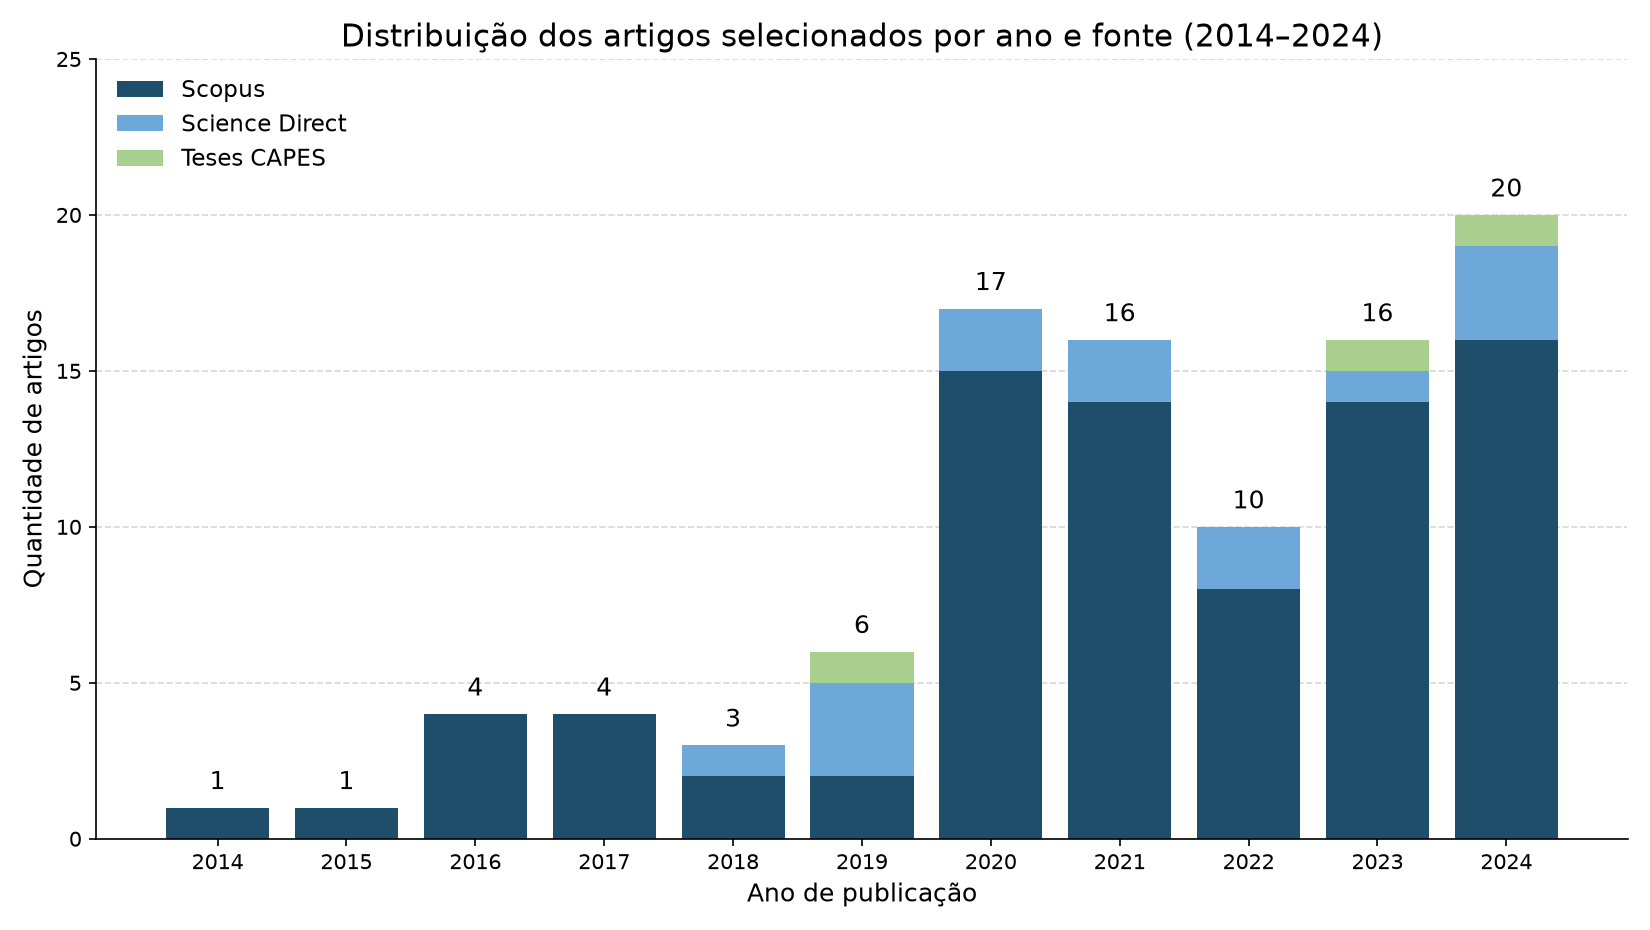
\includegraphics[width=0.95\linewidth]{Imagens/distribuicao_artigos_por_ano_empilhado.png}}{Grafico de barras empilhadas: eixo horizontal lista os anos de 2014 a 2024, eixo vertical indica a quantidade de artigos (escala de 0 a 25), cada barra segmentada por cor conforme a base de origem (Scopus, Science Direct e Catalogo de Teses CAPES). Tendencia de crescimento: 1 artigo em 2014 e 2015, picos de 17 (2020), 16 (2021), 16 (2023) e 20 (2024), com queda pontual para 10 em 2022. Producao incipiente entre 2014 e 2019 (19 trabalhos, 19,4 porcento do corpus), concentrada no bienio 2020-2021 (33 trabalhos, 33,7 porcento) e com crescimento entre 2022 e 2024 (46 trabalhos, 46,9 porcento), com a Scopus predominante em todos os anos (cerca de 82,7 porcento do total).}
    \caption{Distribuição dos 98 artigos do \textit{corpus} por ano e fonte (2014--2024). O gráfico responde à pergunta: como a produção sobre IHD se distribuiu ao longo da última década, por base de dados? É um gráfico de barras empilhadas: o eixo horizontal lista os anos de 2014 a 2024, o eixo vertical indica a quantidade de artigos (escala de 0 a 25), e cada barra é segmentada por cor conforme a base de origem (Scopus, Science Direct e Catálogo de Teses CAPES). A tendência principal é de crescimento: de 1 artigo em 2014 e 2015 para picos de 17 (2020), 16 (2021), 16 (2023) e 20 (2024), com uma queda pontual para 10 em 2022. Em síntese, a produção é incipiente entre 2014 e 2019 (19 trabalhos, 19,4\% do \textit{corpus}), concentra-se no biênio 2020--2021 (33 trabalhos, 33,7\%) e mantém crescimento entre 2022 e 2024 (46 trabalhos, 46,9\%), com a Scopus predominante em todos os anos (cerca de 82,7\% do total).}
    \label{fig:distribuicao_ano_fonte}
\end{figure}

Em contrapartida, as \textbf{170} exclusões concentraram-se em poucos critérios: abordagens superficiais da IHD (\textbf{CE2}) ou o uso do acrônimo em contextos estritamente médicos (\textbf{CE8}) e de \textit{hardware} de baixo nível, desvinculados da interação humana (\textbf{CE4}). A remoção de duplicatas (\textbf{CE9}) e de documentos com barreiras de acesso (\textbf{CE7}) completou o funil. Esse processo de exclusão manteve o \textit{corpus} alinhado ao escopo conceitual da IHD e ao foco em aplicações urbanas.

\subsection{Avaliação de Qualidade dos Estudos}

    Após a etapa de triagem, os \textbf{98} trabalhos do \textit{corpus} final foram submetidos à matriz de avaliação de qualidade, visando avaliar a cobertura de suas contribuições em relação aos temas de interesse da revisão. A inexistência de artigos com pontuação nula é coerente com o critério de seleção adotado, indicando que todas as publicações retidas cobrem ao menos um desses temas.

    A distribuição das avaliações reparte-se por três níveis de cobertura temática, considerando os três pilares conceituais definidos na Seção~\ref{sec:referencial} (legibilidade, agência e negociabilidade) e mais dois eixos analíticos adotados nesta revisão (aplicação em Cidades Inteligentes e gestão de dados do usuário). No estrato superior da Tabela~\ref{tab:resumo_qualidade}, \textbf{41} artigos (41,8\%) alcançaram a pontuação máxima (\textbf{3}). Caracterizados por integrar três ou mais desses eixos de forma articulada, estes estudos combinam, por exemplo, os pilares conceituais da IHD com sua aplicação em contextos urbanos e com a gestão de dados do usuário, servindo de base para as discussões transversais desta revisão. Um grupo de \textbf{27} artigos obteve a pontuação \textbf{2} (27,6\%), relacionando dois desses eixos---tipicamente algum dos pilares conceituais da IHD à sua aplicação prática em contextos urbanos ou à gestão de dados. Por fim, \textbf{30} trabalhos (30,6\%) receberam a pontuação \textbf{1}: abordam um único eixo, com foco em facetas específicas da interação, como transparência e letramento de dados.

    Em suma, a transição da triagem para a avaliação resultou em um referencial bibliográfico que abrange diferentes níveis de cobertura temática. A composição do \textit{corpus}---com estudos que integram três ou mais temas (nível 3), que relacionam dois (nível 2) e que abordam um único eixo (nível 1)---fornece subsídios para a análise do estado da arte.

\section{Resultados e Discussão}
\label{sec:resultados}

A análise dos 98 trabalhos incluídos na Revisão Sistemática permitiu mapear a evolução histórica e estrutural da Interação Humano-Dados (IHD). A documentação completa encontra-se nas \emph{tabelas da RSL}\footnote{Disponível em: https://anonymous.4open.science/r/sbc-rs-4046/Tabelas/. Acesso em: 20 maio 2026.}. Com base na extração sistemática de evidências qualitativas, esta seção apresenta a síntese crítica da literatura, organizada em eixos temáticos que respondem de forma transversal e detalhada às Questões de Pesquisa (QPs e QPSs) delineadas no protocolo metodológico.

\subsection{A Evolução da Gestão de Dados e o Descompasso Sociotécnico (QP1, QP4)}

    Antes da emergência da IHD, a literatura evidencia que as abordagens para a gestão de dados fundamentavam-se em um paradigma predominantemente tecnocrático e centrado na máquina. O foco primário das pesquisas concentrava-se no aprimoramento de tecnologias de Tomada de Decisão Apoiada por Dados (\textit{Data-Supported Decision Making}), priorizando a eficiência do processamento bruto e a segurança algorítmica corporativa em detrimento da carga cognitiva do usuário \cite{calvetti2024human, Locoro2020}. Nesse contexto, o desenvolvimento de \textit{software} operava majoritariamente confinado às camadas física, empírica e sintática da Escada Semiótica (modelo teórico que categoriza os sistemas de informação desde a infraestrutura técnica até o seu impacto no mundo real) \cite{Hornung2015}, negligenciando as dimensões sociais, semânticas e pragmáticas que caracterizam a onipresença informacional na vida cotidiana \cite{Strey2019Human}.

    Nesse período pré-IHD, a proteção informacional ancorava-se no modelo burocrático de ``Aviso e Escolha'' (\textit{Notice and Choice}). Esse mecanismo fundamentava-se na apresentação de termos extensos para a obtenção de um consentimento binário, transferindo a responsabilidade legal ao usuário \cite{Jones2017}. Aliada a isso, havia a imposição de Contratos de Licença de Usuário Final (\textit{End-User License Agreements}---EULAs) que operavam como instrumentos de adesão unilaterais e inegociáveis (\textit{take-it-or-leave-it}). Redigidos em linguagem técnico-jurídica de difícil compreensão, tais contratos condicionavam o acesso ao serviço à aceitação de toda a extração de dados \cite{Hutton2017}.

    A governança da época era regida por marcos regulatórios iniciais, como a Diretiva 95/46/CE,\footnote{Disponível em: https://eur-lex.europa.eu/legal-content/PT/TXT/?uri=CELEX:31995L0046. Acesso em: 20 maio 2026.} antecessora do Regulamento Geral de Proteção de Dados (\textit{General Data Protection Regulation}---GDPR)\footnote{Disponível em: https://eur-lex.europa.eu/legal-content/PT/TXT/?uri=CELEX:32016R0679. Acesso em: 20 maio 2026.}, que regulava o fluxo em uma arquitetura de internet ainda incipiente---e por conceitos estritos de Direito de Propriedade. Essa visão tratava o dado digital, que é altamente replicável e relacional, como um objeto físico isolado, enquadramento inadequado \cite{malgieri2019automated, janecek2018ownership}. Essa abordagem baseada em \textit{walled gardens} (ecossistemas proprietários onde plataformas monopolizam a custódia dos dados e restringem a interoperabilidade) \cite{janecek2018ownership} expôs a racionalidade limitada do ser humano frente à assimetria de poder, bem como à sobrecarga cognitiva gerada por termos de uso extensos \cite{malgieri2020vulnerable, DOWTHWAITE2024, chalhoub2024useful}.
    
    Nesse cenário, a Interação Humano-Computador (IHC) clássica mostrou-se limitada para lidar com as consequências éticas e os riscos sociopsicológicos do processamento de dados invisível e onipresente em rede \cite{Parviainen2016, Calvetti2021173}. Isso porque a área concentrava seus esforços na usabilidade de \textit{hardware} e em métricas de eficiência pontuais, como o tempo de execução de tarefas em telas bidimensionais, sem contemplar a extração ubíqua de rastros digitais.

     A evolução do campo documentada na última década (2014-2024) sinaliza uma transição epistemológica e metodológica. Historicamente, os primeiros estudos que tangenciavam a IHD focavam predominantemente na análise técnica de conjuntos massivos de informações\cite{Parviainen2016, Meireles2016, Hornung2015}. A partir do trabalho fundacional de 2015 \cite{mortier2015humandatainteractionhumanface}, porém, a IHD emerge como campo ético e conceitual autônomo.

    Sob essa nova perspectiva, os dados deixam de ser concebidos como meras entradas passivas do sistema para se tornarem objetos de primeira classe, entidades computacionais autônomas que podem ser manipuladas, transferidas e auditadas diretamente \cite{Crabtree2016}. Consequentemente, esses ativos sociotécnicos passam a exigir tratamento como material de design \cite{seidelin2020foregrounding}, tratando a informação como recurso moldável para mediar a experiência humana, e não como subproduto inerte da programação.

    A prática acadêmica e projetual transita, portanto, da criação de interfaces isoladas para a compreensão de ecossistemas complexos. Essa transição busca integrar o comportamento e as expectativas do indivíduo no ciclo de vida das infraestruturas urbanas, cenário em que o cidadão deixa de ser um espectador técnico e assume o papel de agente ativo, dotado de agência e autonomia \cite{Sailaja2021Designing, bavaresco2019technological}.

    Apesar do potencial dessa virada conceitual, a revisão sistemática revela contrastes e fricções na transição da teoria para a prática implementada. No pilar da \textbf{legibilidade}, a teoria avançou da mera exibição de painéis estáticos (\textit{dashboards}) para a promoção da construção ativa de sentido (\textit{data sensemaking}), estruturada em eixos de inspeção, engajamento e contextualização da informação \cite{Koesten2021}. Contudo, as implementações reais em ecossistemas digitais ainda apresentam jargões técnicos de difícil compreensão e fluxos de decisão não lineares \cite{Sailaja2021}.

    No pilar da \textbf{agência}, o conceito evoluiu da aceitação de modelos de consentimento binários para arquiteturas de prestação de contas (\textit{accountability}) \cite{janecek2018ownership}. Nesses novos paradigmas sociotécnicos, o cidadão passa a dispor de mecanismos concretos para rastrear o fluxo informacional, auditar decisões algorítmicas e exigir justificativas claras, sendo promovido à figura de administrador (\textit{steward}) de seus próprios rastros digitais \cite{angelopoulos2021stewardship}. 

    Todavia, a revisão indica que projetistas e desenvolvedores enfrentam barreiras na prática. Sem o suporte metodológico de diretrizes operacionais ou heurísticas validadas, torna-se complexo aplicar esses artefatos teóricos durante o desenvolvimento de \textit{software} \cite{Strey2019Human, Victorelli2020Human, chalhoub2024useful}. 

    Por fim, a \textbf{negociabilidade} expandiu-se das interações mediadas por telas para a governança difusa de dados capturados ininterruptamente por sensores urbanos (IoT), frequentemente sem engajamento consciente do transeunte \cite{Locoro2020}. Contudo, a efetivação dessa dimensão na prática urbana depara-se com a fragmentação das ferramentas de controle, o que compromete um diálogo simétrico e participativo entre a população e os sistemas que a monitoram \cite{Chatzimichali2021160}.
        
    \subsection{Lacunas Estruturais, Desafios Cognitivos e Opacidade (QP2, QP3)}

    A análise do acervo selecionado revela que a IHD, embora conceitualmente estruturada, ainda enfrenta lacunas estruturais que dificultam sua implementação em larga escala \cite{Sailaja2021Designing, Strey2019Human}. Persiste a falta de um paradigma produtivo consolidado e a carência de um conjunto de heurísticas de \textit{design} validadas para orientar desenvolvedores em domínios específicos, com destaque para o contexto de geoprocessamento \cite{Capeleti2024Human}. Ademais, a literatura ainda apresenta ambiguidades na definição dos perfis e do usuário final das plataformas de dados urbanos \cite{Belizario2023Interacao} e carece de especificações técnicas sobre o que torna um conjunto de dados abertos efetivamente reutilizável \cite{Koesten2020}.

    Uma lacuna frequentemente negligenciada refere-se à sobrecarga cognitiva imposta aos usuários \cite{Locoro2020}. A literatura aponta um impacto sociopsicológico negativo decorrente da onipresença informacional, manifesto na fadiga cognitiva e na ansiedade informacional decorrente da perda de controle sobre a destinação de seus registros pessoais \cite{cezar2023cognitive}.

    Lockwood \cite{Lockwood2021, Lockwood2020AnAccessible} destaca, por exemplo, a ausência de modelos mentais maduros para lidar com tecnologias emergentes, como a Identidade Autossoberana (\textit{Self-Sovereign Identity}---SSI). Esse paradigma de arquitetura digital descentralizada foi estruturado para permitir que o cidadão gerencie autonomamente suas próprias credenciais, sem depender de provedores centrais. No entanto, sua operação ainda se revela excessivamente complexa para o público leigo \cite{Lockwood2021, Lockwood2020AnAccessible}. Consequentemente, o autor aponta que persiste uma escassez de estudos que cruzem a visão técnica dos especialistas em engenharia com a percepção de usabilidade e o modelo mental do cidadão comum \cite{Lockwood2020AnAccessible}.

   A integração ética com Inteligência Artificial e algoritmos corporativos emerge como outra área de vulnerabilidade apontada pela literatura. Sistemas de análise visual baseados em aprendizado de máquina para dados de redes sociais em tempo real, por exemplo, enfrentam vieses e incertezas decorrentes de mudanças na distribuição dos dados (\textit{covariate shift}), dificultando o \textit{sensemaking} humano sobre os fluxos de informação \cite{Haghighati2020}. Além disso, a legibilidade algorítmica esbarra recorrentemente no sigilo industrial e na opacidade das caixas-pretas corporativas, comprometendo o Direito à Explicação das decisões automatizadas que afetam a rotina do cidadão \cite{Barreto2018} \cite{DeAlmeida2019}.

    No âmbito das plataformas de gestão, a literatura evidencia a ineficácia prática dos atuais \textit{Personal Data Management Services} (Serviços de Gestão de Dados Pessoais---PDMS)---repositórios onde o indivíduo deveria centralizar o controle de suas informações---em conciliar a pressão comercial do extrativismo de dados com a real preservação da agência do usuário \cite{angelopoulos2021stewardship}.

    Por fim, a transposição empírica dos princípios da IHD para comunidades desfavorecidas constitui um desafio ainda não superado: a dataficação frequentemente exacerba as disparidades digitais pré-existentes \cite{hayes2024making, Locoro2020}. O equilíbrio entre a otimização de serviços em Cidades Inteligentes e a proteção da privacidade permanece classificado como um ``problema perverso''---interdependente, sistêmico e sem solução puramente técnica \cite{Meireles2016, Chowdhury2016}. As diretrizes de controle vigentes mostram-se limitadas diante da capilaridade da infraestrutura urbana, restringindo a capacidade do cidadão de discernir o propósito desse monitoramento passivo \cite{Mashhadi2014}.


    \subsection{IHD em Cidades Inteligentes: Capacidade Cívica e Fatores Culturais (QP5, QPS4)}

    A aplicação da IHD no ecossistema de Cidades Inteligentes (\textit{Smart Cities}) contribui para o enfrentamento dos desafios emergentes relativos à gestão informacional e à participação cidadã. Como os ambientes urbanos geram vastos volumes de dados a partir de sensores e dispositivos de Internet das Coisas (IoT), a IHD estabelece a conexão conceitual com essa infraestrutura, propondo modelos de governança específicos para o tecido urbano \cite{Mashhadi2014, Chowdhury2016, barcellos2022towards}.

    Em vez de se limitar à automação técnica, essa perspectiva emprega a computação cívica e abordagens de tecnologia calma (\textit{calm technology}) para monitorar o ambiente de forma não intrusiva, visando ao bem-estar local e à segurança ciberfísica, desde que a arquitetura do sistema respeite a privacidade como premissa central \cite{Konomi2022, Chowdhury2016}.

    No contexto da governança urbana, a \textbf{legibilidade} é fundamental para que os habitantes compreendam a coleta contínua efetuada por sensores de rua \cite{Coleti2019DesigPatterns, Hutton2017}. A IHD revela o espectro que une atos cotidianos (como o uso do transporte público) às macroestruturas de extração global, conferindo capacidade cívica para que o morador entenda plataformas de segurança em situações de crise. O objetivo central é fomentar o questionamento crítico, reconhecendo que dados abertos raramente são politicamente neutros \cite{Parviainen2016, barcellos2022towards}.

    Contudo, a efetivação dessa legibilidade esbarra em barreiras idiomáticas e culturais. A literatura destaca, por exemplo, o impacto do viés de legado (\textit{legacy bias})---fenômeno em que os usuários tendem a reproduzir comportamentos condicionados por tecnologias que já conhecem \cite{Friedman2024}. Para superar esse obstáculo, exige-se a adaptação de metáforas visuais ao contexto local, utilizando metodologias inclusivas como o \textit{HDIdea} (focado no entendimento sistêmico por parte do usuário) \cite{Strey2019Human} e o \textit{framework} ATLAS (voltado à avaliação de sistemas de geoinformação) \cite{Capeleti2024Human}.

    A \textbf{agência} refere-se à capacidade de controle sobre rastros digitais em espaços fisicamente saturados de conectividade. A reversão do quadro de impotência do usuário demanda o gerenciamento descentralizado e o processamento local de informações \cite{Sailaja2021, Crabtree2016}. Nesse cenário, a IHD atua como salvaguarda democrática ao exigir a Limitação da Finalidade, garantindo que a confiança cidadã se sustente no direito de desativar a captura ambiental e de aprovar os usos secundários da informação \cite{Mashhadi2014}.

    O exercício desse controle é modulado por fatores culturais: culturas coletivistas apresentam maior aceitação do compartilhamento informacional voltado ao benefício coletivo, ao passo que culturas individualistas priorizam a restrição pessoal \cite{Locoro2020}. No contexto brasileiro---cenário caracterizado por históricas assimetrias socioeconômicas e disparidades agudas de letramento digital---a importação acrítica de modelos de governança desenhados sob os valores do Norte Global pode acentuar o impacto do viés de legado \cite{Friedman2024}. Simultaneamente, minorias étnicas, marcadas por um histórico de estratificação social, mostram-se reticentes em negociar seus dados com o Estado. Consequentemente, grupos vulneráveis são frequentemente alijados do processo de \textit{sensemaking}, ficando expostos a um risco acrescido de discriminação algorítmica e exclusão das dinâmicas das Cidades Inteligentes \cite{malgieri2020vulnerable, Yuan20243615}.

    Por fim, a \textbf{negociabilidade} exige que a infraestrutura municipal, a exemplo dos edifícios inteligentes (\textit{Smart Buildings}), responda dinamicamente às preferências de privacidade do cidadão \cite{bavaresco2019technological, Brombacher20221863}. Esse engajamento varia conforme a geografia e a confiança institucional, aspecto discutido no contexto brasileiro a partir da interação de cidadãos não especialistas com plataformas de dados em Cidades Inteligentes \cite{Belizario2023Interacao}. Para mitigar esse descompasso empírico e viabilizar uma negociabilidade real, evidencia-se o esforço da comunidade brasileira de Fatores Humanos em Sistemas Computacionais (IHC) em adaptar \textit{frameworks} de avaliação \cite{Belizario2023Interacao, Victorelli2020Human, barcellos2022towards}. Essa adaptação geopoliticamente situada dialoga com os Grandes Desafios de Pesquisa (GranDIHC-BR 2025-2035) \cite{Pereira}. O planejamento urbano poderia priorizar abordagens não extrativistas, usando a Inteligência Artificial Generativa para preservar as ``histórias humanas'' subjacentes às métricas \cite{ferreira2024connecting}.
    
    %No entanto, o exercício desse controle é profundamente modulado por fatores ligados ao eixo autonomia-coletivismo. Em culturas coletivistas, observa-se maior aceitação do compartilhamento informacional voltado ao benefício coletivo, ao passo que culturas individualistas priorizam a restrição pessoal \cite{Locoro2020}. Simultaneamente, minorias étnicas, marcadas por um histórico de estratificação social, mostram-se reticentes em negociar seus dados com o Estado, o que coloca grupos vulneráveis em risco acrescido de discriminação algorítmica e exclusão \cite{Yuan20243615, Lenzi2024, malgieri2020vulnerable, chalhoub2024useful, Parviainen2016}.

    %Por fim, a \textbf{negociabilidade} exige que a infraestrutura municipal, a exemplo dos edifícios inteligentes (\textit{Smart Buildings}), responda dinamicamente às preferências de privacidade do cidadão \cite{DOWTHWAITE2024, Nelson2023, bavaresco2019technological, Elhamdadi2022, Xiao2021, Koesten2021, Sailaja2024334, Chowdhury2016, Seidelin2018}. Esse engajamento varia conforme a geografia e a confiança institucional; nota-se que os moradores se envolvem mais ativamente com informações hiperlocais quando o sistema respeita suas normativas socioculturais. O planejamento urbano deve, portanto, rejeitar matrizes extrativistas e utilizar a tecnologia (como a Inteligência Artificial Generativa) para preservar as ``histórias humanas'' inerentes às métricas, consolidando uma urbanização transparente e resiliente \cite{Briggs2021, Sailaja2021, Jandric2023, Belizario2023Interacao, calvetti2024human, Calvetti2021173, Stead2022, Turkay2021, coleti2024humanSillabus, Refat2023, Chatzimichali2021160}.

    \subsection{Avaliação Metodológica, Validação de \textit{Frameworks} e Inclusão Digital (QPS1, QPS2, QPS3)}

    A materialização da IHD exige a tradução de construtos teóricos em interfaces acessíveis, atenuando as assimetrias de acesso para usuários com baixo letramento digital. Historicamente, a literatura apoiou-se em heurísticas clássicas como o ``Mantra de Shneiderman''---que prioriza a visão geral do sistema, seguida por ferramentas de \textit{zoom} e filtro---abordagem útil para organizar painéis visuais \cite{Victorelli2020Human}. Contudo, investigações recentes contrapõem essa visão, argumentando que a mera organização espacial é insuficiente para o público leigo \cite{Yuan20243615, Lindley2020}.

    Para suprir essa deficiência, o campo tem migrado para estratégias de \textit{design} inclusivo fundamentadas em modelos mentais pré-existentes, que empregam semânticas visuais familiares ao usuário \cite{Barreto2018, DeAlmeida2019}. O estado da arte aponta que uma das estratégias mais promissoras para democratizar a construção de sentido é o suporte progressivo ao aprendizado (\textit{scaffolding}), que substitui sintaxes complexas por questionamentos guiados \cite{Trajkova2020}.

    Para romper a fadiga imposta por telas, a literatura evidencia uma guinada multissensorial. Por um lado, as Interfaces de Voz (VUI) e a sonificação reduzem o esforço de aprendizado ao aproveitar vias auditivas e vieses motores legados (como o movimento de pinça em dispositivos móveis) \cite{Sailaja2021, Friedman2024}. Por outro lado, interações efêmeras dificultam a retenção de termos contratuais \cite{Jones2017, Lockwood2021}. 

    Como contraponto à abstração das interações efêmeras, ganha força a fisicalização tátil e o uso de \textit{Databoxes} (nós de processamento local). Essas soluções convertem a governança em uma relação tangível, viabilizando os ``Mercados de Dados'' (\textit{Data Marketplaces}) \cite{Crabtree2016}. Aliados a isso, o uso de cronologias interativas (\textit{timelines}) é apontado como alternativa aos painéis tradicionais para explicitar períodos de retenção, cuja explicabilidade permanece limitada nas soluções atuais \cite{DeAlmeida2019}.

    A estruturação desses elementos apoia-se na validação empírica de \textit{frameworks} arquiteturais. O modelo de \cite{mortier2015humandatainteractionhumanface} permanece como lente analítica primária, testado clinicamente \cite{sailaja2021exploring} e em veículos conectados \cite{DOWTHWAITE2024}. 

    Para transpor a teoria abstrata à prática de \textit{design}, surgiram \textit{frameworks} contextuais e híbridos. O HDIdea (\textit{Human-Data Ideation}) integra o Diagrama de Partes Interessadas e a Escada Semiótica para avaliar o impacto pragmático \cite{Strey2019Human}; e o ATLAS consolida heurísticas para mapas interativos \cite{Capeleti2024Human}. Nota-se também uma hibridização da IHD com a Teoria Institucional \cite{mu2024institutional}, Sistemas Ciberfísicos (CPS) \cite{bavaresco2019technological, Zou2020769} e Inteligência Artificial Explicável (XAI) \cite{Yuan20243615, Turkay2021, durango2024data}, demonstrando a plasticidade da área.

    Por fim, a mensuração dessas arquiteturas exige métodos mistos. Para avaliar a sobrecarga cognitiva subconsciente, os estudos priorizam o \textit{eye-tracking}, útil em painéis complexos \cite{Capeleti2024Human, kaufmann2021ethical}. Em contrapartida, para aferir a compreensão cívica de forma pragmática, os estudos aplicam o protocolo \textit{Think-Aloud}, avaliações heurísticas colaborativas, entrevistas em profundidade com peritos e o Método de Avaliação de Comunicabilidade (MAC), além de questionários estruturados para medir a utilidade percebida \cite{Strey2019Human, Belizario2023Interacao, Capeleti2024Human}. 

    O uso de testes A/B, Mapeamentos Sistemáticos e painéis \textit{Delphi} fundamenta o consenso acadêmico contínuo \cite{calvetti2024human, hayes2024making, Refat2023}. A comunidade brasileira de Fatores Humanos em Sistemas Computacionais tem nacionalizado esses protocolos, convertendo-os em ferramentas contra as disparidades da dataficação no contexto nacional \cite{Capeleti2024Human, Strey2019Human, Belizario2023Interacao}.

    A Tabela \ref{tab:matriz_frameworks} sintetiza o cruzamento estrutural entre os principais \textit{frameworks} mapeados, seus contextos de validação urbana empírica e o respectivo arsenal metodológico empregado.


\begin{table}[H] % Alterado de [H] para [htb] para permitir que o LaTeX gerencie a flutuação de forma mais fluida
\centering
\caption{Matriz Comparativa: Frameworks, Validação Empírica e Métodos de Avaliação em IHD}
\label{tab:matriz_frameworks}
\scriptsize
\renewcommand{\arraystretch}{1.0}
\setlength{\tabcolsep}{3pt}
\begin{tabular}{
  >{\raggedright\arraybackslash}p{0.22\linewidth}
  >{\raggedright\arraybackslash}p{0.30\linewidth}
  >{\raggedright\arraybackslash}p{0.18\linewidth}
  >{\raggedright\arraybackslash}p{0.22\linewidth}
}
\toprule
\textbf{Abordagem / Framework} & \textbf{Contexto Urbano / Validação Empírica} & \textbf{Princípio Coberto} & \textbf{Método de Avaliação} \\ \midrule
\textbf{Modelo Fundacional \cite{mortier2015humandatainteractionhumanface}} & Ecossistemas de saúde e coleta de telemetria em veículos conectados. & Legibilidade, Agência, Negociabilidade. & Testes clínicos, questionários estruturados e estudos de caso. \\
\textbf{HDIdea (\textit{Human-Data Ideation}) \cite{Strey2019Human}} & Fase de ideação semiótica e concepção de \textit{software} focado no impacto pragmático. & Legibilidade. & \textit{Think-Aloud}, heurísticas colaborativas e entrevistas com peritos. \\
\textbf{ATLAS (Geoprocessamento) \cite{Capeleti2024Human}} & Plataformas governamentais de mapas interativos e dados abertos locais. & Legibilidade e Agência. & \textit{Eye-tracking}, Método de Avaliação de Comunicabilidade (MAC). \\
\textbf{\textit{Databoxes} e Mercados de Dados \cite{Crabtree2016}} & Processamento local em \textit{Smart Buildings} e governança residencial descentralizada. & Agência e Negociabilidade. & Testes A/B, prototipação tangível e cronologias interativas (\textit{timelines}). \\
\textbf{IHD Multissensorial (VUI e Tátil) \cite{Sailaja2021, Friedman2024, Crabtree2016}} & Espaços públicos interativos voltados a populações com baixo letramento técnico. & Legibilidade (foco em Acessibilidade). & Observação de vieses motores, painéis \textit{Delphi} e avaliações comportamentais. \\
\textbf{Diretrizes Cognitivas (\textit{Scaffolding}) \cite{Trajkova2020}} & Tradução de sintaxes complexas para o público leigo via questionamentos guiados. & Legibilidade (Sensemaking). & Mapeamentos sistemáticos e testes de usabilidade clássicos. \\
\textbf{Modelos Híbridos (CPS e XAI) \cite{bavaresco2019technological, durango2024data}} & Auditoria de caixas-pretas algorítmicas na infraestrutura municipal. & Agência e Negociabilidade. & Validação teórica cruzada (Teoria Institucional). \\ \bottomrule
\end{tabular}
\end{table}

    Como contribuição desta revisão, propomos uma taxonomia que situa os \textit{frameworks} da Tabela 5 nos três pilares do Modelo Fundacional \cite{mortier2015humandatainteractionhumanface}, sintetizada na Tabela 6. ATLAS e \textit{Databoxes}/Modelos Híbridos aparecem em mais de um pilar por cobrirem princípios sobrepostos; os eixos de aplicação em Cidades Inteligentes e gestão de dados do usuário, usados na avaliação de qualidade, permanecem como dimensões de pontuação, sem \textit{frameworks} próprios mapeados.

\begin{table}[H]
\centering
\caption{Taxonomia de \textit{Frameworks} por Pilar da IHD}
\label{tab:taxonomia_ihd}
\scriptsize
\renewcommand{\arraystretch}{1.0}
\setlength{\tabcolsep}{3pt}
\begin{tabular}{
  >{\raggedright\arraybackslash}p{0.16\linewidth}
  >{\raggedright\arraybackslash}p{0.30\linewidth}
  >{\raggedright\arraybackslash}p{0.46\linewidth}
}
\toprule
\textbf{Pilar} & \textbf{Definição} & \textbf{\textit{Frameworks} mapeados (método de avaliação)} \\ \midrule
\textbf{Legibilidade} & Capacidade do usuário de compreender e construir sentido sobre os dados coletados. & HDIdea (\textit{Think-Aloud}, heurísticas, entrevistas); ATLAS (\textit{eye-tracking}, MAC); IHD Multissensorial (vieses motores, Delphi); Diretrizes Cognitivas/\textit{Scaffolding} (mapeamentos sistemáticos, usabilidade). \\
\textbf{Agência} & Papel ativo do cidadão como administrador de seus próprios rastros digitais. & ATLAS (\textit{eye-tracking}, MAC); \textit{Databoxes} e Mercados de Dados (testes A/B, prototipação tangível); Modelos Híbridos CPS/XAI (validação teórica cruzada). \\
\textbf{Negociabilidade} & Revisão e revogação dinâmica de permissões conforme o contexto se transforma. & \textit{Databoxes} e Mercados de Dados (testes A/B, prototipação tangível); Modelos Híbridos CPS/XAI (validação teórica cruzada). \\ \bottomrule
\end{tabular}
\end{table}

    Para consolidar as discussões transversais levantadas nesta revisão, a Tabela \ref{tab:sintese_geral} apresenta um mapeamento panorâmico do estado da arte, conectando as Questões de Pesquisa aos principais achados sociotécnicos discutidos.

\begin{table}[H]
\centering
\caption{Síntese do Estado da Arte em Interação Humano-Dados (2014-2024)}
\label{tab:sintese_geral}
\small
\begin{tabular}{p{0.15\linewidth} p{0.25\linewidth} p{0.50\linewidth}}
\hline
\textbf{Questões (QPs)} & \textbf{Eixo Temático} & \textbf{Principais Achados e Lacunas Sistêmicas} \\ \hline
\textbf{QP1, QP4} & Evolução e Paradigmas & Transição da viabilidade técnica (IHC clássica) para a complexidade sociotécnica. Superação do modelo burocrático de ``Aviso e Escolha'' (\textit{Notice and Choice}) para o tratamento do dado como objeto de primeira classe. \\ \hline
\textbf{QP2, QP3} & Lacunas e Descompasso Prático & Hiato entre a teoria da agência e a prática de mercado. A carência de heurísticas validadas gera interfaces opacas que impõem sobrecarga cognitiva e ansiedade informacional aos usuários. \\ \hline
\textbf{QP5, QPS4} & Cidades Inteligentes e Fatores Culturais & A IHD atua como salvaguarda contra a vigilância urbana, conferindo capacidade cívica. A efetividade exige mitigar barreiras idiomáticas e o viés de legado, respeitando assimetrias entre culturas coletivistas e individualistas. \\ \hline
\textbf{QPS1 a QPS3} & Avaliação e Inclusão Multissensorial & Aplicação de métodos mistos (Heurísticas, MAC, \textit{Eye-tracking}). Para o público leigo, a mitigação da abstração via fisicalização tátil, \textit{Databoxes} e Interfaces de Voz (VUI) é indicada para democratizar a construção ativa de sentido (\textit{data sensemaking}). \\ \hline
\end{tabular}
\end{table}

    Conforme sintetizado, a diversidade de desafios e a evolução metodológica adotada pelos estudos recentes reforçam a necessidade de abordagens híbridas para avaliar a Interação Humano-Dados de forma abrangente. A transição de métodos estritamente técnicos (como testes clássicos de usabilidade em tela) para estratégias de inclusão multissensorial (como a fisicalização tátil e o uso de \textit{Databoxes}) evidencia um esforço acadêmico expressivo para mitigar a exclusão digital. 

    Consequentemente, esse arsenal estrutural sugere que a governança de dados no contexto de \textit{Smart Cities} tende a se tornar mais democrática à medida que o \textit{design} de \textit{software} transcender as métricas tradicionais da IHC. Isso exige um foco ativo na redução da ansiedade de dados, no respeito às singularidades culturais e na tradução de infraestruturas invisíveis em interfaces que sejam, de fato, operáveis pelo cidadão comum.

    \section{Ameaças à Validade}
    \label{sec:ameacas}

    A condução deste mapeamento sistemático seguiu o protocolo de \cite{KITCHENHAM2013} visando conferir transparência ao processo. Contudo, é fundamental reconhecer ameaças inerentes ao método que podem delimitar o alcance dos achados.

    No que tange à \textbf{validade interna}, esta pesquisa reconhece o viés subjetivo inerente às etapas de triagem e extração, conduzidas pelos dois autores deste trabalho, mas sem um protocolo formal de dupla triagem cega e independente para conciliação de casos de fronteira. A decisão de incluir ou excluir um artigo---especialmente na aplicação de critérios que exigem julgamento de valor, como a distinção entre uma ``contribuição teórica robusta'' e uma ``menção superficial'' (CE2)---é influenciada pela perspectiva individual, mitigada pela escoragem sistemática da Avaliação de Qualidade (Tabela~\ref{tab:qualidade}), cujos artefatos de pontuação por artigo estão documentados no repositório suplementar e podem ser auditados externamente.

    Quanto à \textbf{validade de constructo}, a principal ameaça reside na especificidade da \textit{string} de busca. Embora o termo ``Human-Data Interaction'' seja o descritor central da área, sua escolha como eixo principal pode ter omitido estudos que discutem princípios análogos (como agência e legibilidade) sob outras nomenclaturas (ex.: ``user-centric data'' ou ``soberania digital''), dada a fluidez terminológica de um campo interdisciplinar em consolidação. Cabe destacar que essa omissão não decorre necessariamente de uma limitação da indexação da Scopus em si, mas sim da recuperabilidade de um estudo frente a uma \textit{string} de busca específica: um trabalho tecnicamente indexado pode não ser retornado por uma consulta \textit{TITLE-ABS-KEY} se seus autores tiverem optado por terminologia distinta da adotada nesta revisão. Essa lacuna, portanto, não é atribuível à qualidade do estudo original nem a uma escolha editorial deliberada de seus autores em relação aos metadados, mas a uma característica estrutural de campos interdisciplinares em consolidação terminológica, na qual conceitos correlatos coexistem sob rótulos distintos.

    Por fim, a \textbf{validade externa} é delimitada pela exclusão deliberada de literaturas cinzentas, consequência direta do critério \textbf{CI7} (revisão por pares) e do protocolo de RSL adotado \cite{KITCHENHAM2013}, que priorizam o rigor e a replicabilidade da síntese em detrimento da cobertura de fontes não revisadas. Esse recorte, padrão em revisões sistemáticas, pode ter deixado de fora evidências práticas contidas em relatórios técnicos governamentais ou \textit{white papers} de tecnologia, relevantes para o contexto de Cidades Inteligentes. O reconhecimento dessa delimitação não invalida o \textit{corpus} de 98 estudos, mas delimita o alcance das generalizações propostas.

    \subsection{Limitações do Estudo}

    Distintamente das ameaças à validade, que dizem respeito a riscos ao rigor metodológico da própria condução da RSL, as limitações aqui descritas referem-se ao alcance e à profundidade do escopo definido para esta pesquisa. Em primeiro lugar, a opção pela Scopus como base principal, embora justificada pela padronização da extração de metadados (Seção~3.1), restringe a cobertura de trabalhos indexados exclusivamente em repositórios nativos (ACM Digital Library, IEEE Xplore) ou em plataformas nacionais de acesso aberto como a SOL. Em segundo lugar, a taxonomia proposta na Tabela 6 organiza apenas os \textit{frameworks} explicitamente mapeados nesta RSL pelos três pilares do Modelo Fundacional, sem pretensão de exaustividade; sua consolidação em uma taxonomia estruturada da IHD em contextos urbanos, validada por especialistas e estendida a novos \textit{frameworks}, permanece um trabalho futuro promissor.

    \section{Conclusão}

    Este artigo apresentou um mapeamento sistemático da literatura sobre a Interação Humano-Dados (IHD) no decênio 2014-2024, analisando sua evolução no contexto das cidades inteligentes. A investigação de um \textit{corpus} de 98 estudos permitiu observar que, embora os pilares de legibilidade, agência e negociabilidade possuam fundação teórica consolidada, sua materialização para sistemas urbanos reais parece marcada por um hiato considerável. As evidências sugerem que as implementações atuais ainda priorizam a eficiência técnica em detrimento da soberania do sujeito, associando-se a fenômenos como a fadiga do consentimento e a ansiedade de dados.

    A contribuição deste trabalho reside na sistematização das lacunas sociotécnicas e do arcabouço metodológico que impactam a governança democrática de dados. Os achados sugerem que a eficácia da IHD não depende apenas de transparência algorítmica, mas também de um \textit{design} que reconheça as assimetrias de letramento digital e os fatores étnico-culturais. A análise aponta que estratégias inclusivas, como a fisicalização de dados, o suporte progressivo (\textit{scaffolding}) e o uso de narrativas (\textit{storytelling}), surgem como caminhos promissores para reduzir o abismo entre a infraestrutura invisível das \textit{Smart Cities} e a percepção humana.

    Como direcionamento para trabalhos futuros, os achados e a matriz comparativa deste mapeamento podem servir de subsídio para uma investigação empírica situada. Como etapa subsequente, a pesquisa buscará explorar as tensões teóricas aqui identificadas por meio da análise empírica de aplicativos urbanos de amplo uso no contexto da cidade de São Paulo. O objetivo consistirá na proposição de diretrizes de \textit{design} que busquem mitigar o viés de legado. Desse modo, esta pesquisa contribui para uma interação informacional mais equitativa, transparente e humanizada, em diálogo com os Grandes Desafios de Pesquisa em Interação Humano-Computador no Brasil (GranDIHC-BR-2025-2035) e com as demandas do ecossistema sociotécnico nacional.

    %Este artigo consolidou um mapeamento sistemático da literatura sobre a Interação Humano-Dados (IHD) no decênio 2014-2024, analisando o amadurecimento desse campo crítico no contexto das cidades inteligentes. A investigação de um \textit{corpus} de 102 estudos permitiu diagnosticar que, embora os pilares de legibilidade, agência e negociabilidade possuam uma fundação teórica robusta, sua materialização para sistemas urbanos reais é marcada por um hiato profundo. As evidências revelam que as implementações atuais ainda priorizam a eficiência técnica em detrimento da soberania do sujeito, resultando em fenômenos como a fadiga do consentimento e a ansiedade de dados.

    %A contribuição central deste trabalho reside na sistematização das lacunas sociotécnicas que impedem uma governança democrática de dados. Reiteramos que a eficácia da IHD não depende apenas de transparência algorítmica, mas de um \textit{design} que reconheça as assimetrias de letramento digital e os fatores étnico-culturais. A análise aponta que estratégias como a fisicalização de dados e o uso de narrativas (\textit{storytelling}) surgem como caminhos promissores para reduzir o abismo entre a infraestrutura invisível das \textit{Smart Cities} e a percepção humana.

    %Como direcionamento para trabalhos futuros, os achados deste mapeamento servirão de alicerce para uma investigação empírica situada. Como etapa subsequente, a pesquisa buscará validar as tensões teóricas aqui identificadas por meio da análise empírica de aplicativos urbanos de amplo uso no contexto da cidade de São Paulo. O objetivo primário consistirá na proposição de diretrizes de \textit{design} capazes de mitigar o viés de legado (\textit{legacy bias}). Desse modo, almeja-se promover uma interação informacional mais equitativa, transparente e humanizada, intrinsecamente alinhada às singularidades e às demandas do ecossistema sociotécnico brasileiro.


    \section*{Cuidados Éticos}

    Não aplicável. Este trabalho é uma Revisão Sistemática da Literatura, sem coleta de dados com seres humanos.

    \section*{Agradecimentos}

    Seção omitida para fins de revisão duplo-cega. Os agradecimentos institucionais, de financiamento e pessoais serão incluídos na versão final do artigo.
    %Agradeço ao Programa de Pós-Graduação em Sistemas de Informação, da instituição anônima, pelo suporte institucional. %O presente trabalho foi realizado com o apoio da Coordenação de Aperfeiçoamento de Pessoal de Nível Superior - Brasil (CAPES) - Código de Financiamento Anônimo. 
    %O presente trabalho foi realizado com o apoio de agência de fomento nacional---Código de Financiamento Anônimo. Expresso também minha profunda gratidão ao meu esposo Anônimo, e ao meu filho Anônimo, pelo amor, compreensão e suporte incondicional, que foram a base fundamental para que a realização deste artigo fosse possível.

    Por fim, em conformidade com as diretrizes de transparência da conferência, declaro que, durante a preparação deste documento, utilizei a Inteligência Artificial Generativa \textit{Gemini 3.1 Pro} (\textit{Google}) e \textit{Claude Opus 4.7} (\textit{Anthropic}) com o propósito exclusivo de refinamento gramatical, aprimoramento da fluidez textual e estruturação sintática dos textos e da tabela de síntese. %Ressalto que a concepção original das ideias, a condução da revisão sistemática, a seleção do referencial teórico, a análise crítica e as conclusões apresentadas são de minha autoria e responsabilidade. Todo o conteúdo que recebeu apoio ferramental de inteligência artificial foi criteriosamente revisado, editado e validado quanto à sua precisão científica, originalidade e aderência à literatura de Interação Humano-Dados.


\bibliographystyle{sbc}
\bibliography{Referencias/referencias}

\end{document}
